\documentclass{article}
\usepackage[fleqn]{amsmath}
\usepackage{amssymb}
\usepackage{algorithm}
\usepackage{algpseudocode}
\usepackage{enumitem}
\usepackage{listings}
\usepackage{xcolor}
\usepackage{apacite}
\usepackage{svg}
\usepackage{placeins}
\usepackage{float}
\usepackage[margin=1in]{geometry}
\usepackage{lipsum}
\usepackage{textcomp}
\usepackage{graphicx}
\usepackage{url}
\usepackage{lipsum}

\newcommand\tab[1][1cm]{\hspace*{#1}}
\newenvironment{bottompar}{\par\vspace*{\fill}}{\clearpage}
% \usepackage{showframe}

% \newcommand*{\SignatureAndDate}[1]{
%     \par\noindent\makebox[2.5in]{\hrulefill}
%     \hfill\makebox[2.0in]{\hrulefill}
%     \par\noindent\makebox[2.5in][l]{#1}
%     \hfill\makebox[2.0in][l]{Date}
% }

\graphicspath{{./Images/}}

\definecolor{listinggray}{gray}{0.9}
\definecolor{lbcolor}{rgb}{0.9,0.9,0.9}
\definecolor{darkgreen}{rgb}{0.0, 0.2, 0.13}
\definecolor{mygreen}{RGB}{28,172,0} % color values Red, Green, Blue
\definecolor{mylilas}{RGB}{170,55,241}
\lstset{
backgroundcolor=\color{lbcolor},
    tabsize=4,    
%   rulecolor=,
    language=[GNU]C++,
        basicstyle=\scriptsize,
        upquote=true,
        aboveskip={1.5\baselineskip},
        columns=fixed,
        showstringspaces=false,
        extendedchars=false,
        breaklines=true,
        prebreak = \raisebox{0ex}[0ex][0ex]{\ensuremath{\hookleftarrow}},
        frame=single,
        numbers=left,
        showtabs=false,
        showspaces=false,
        showstringspaces=false,
        identifierstyle=\ttfamily,
        keywordstyle=\color[rgb]{0,0,1},
        commentstyle=\color[rgb]{0.026,0.112,0.095},
        stringstyle=\color[rgb]{0.627,0.126,0.941},
        numberstyle=\color[rgb]{0.205, 0.142, 0.73},
%        \lstdefinestyle{C++}{language=C++,style=numbers}’.
}
% \lstset{
%     backgroundcolor=\color{lbcolor},
%     tabsize=4,
%   language=C++,
%   captionpos=b,
%   tabsize=3,
%   frame=lines,
%   numbers=left,
%   numberstyle=\tiny,
%   numbersep=5pt,
%   breaklines=true,
%   showstringspaces=false,
%   basicstyle=\footnotesize,
% %  identifierstyle=\color{magenta},
%   keywordstyle=\color[rgb]{0,0,1},
%   commentstyle=\color{darkgreen},
%   stringstyle=\color{red}
%   }

\lstset{language=Matlab,%
    %basicstyle=\color{red},
    breaklines=true,%
    morekeywords={matlab2tikz},
    keywordstyle=\color{blue},%
    morekeywords=[2]{1}, keywordstyle=[2]{\color{black}},
    identifierstyle=\color{black},%
    stringstyle=\color{mylilas},
    commentstyle=\color{mygreen},%
    showstringspaces=false,%without this there will be a symbol in the places where there is a space
    numbers=left,%
    numberstyle={\tiny \color{black}},% size of the numbers
    numbersep=9pt, % this defines how far the numbers are from the text
    emph=[1]{for,end,break},emphstyle=[1]\color{red}, %some words to emphasise
    %emph=[2]{word1,word2}, emphstyle=[2]{style},    
}

% \setcounter{biburllcpenalty}{7000}
% \setcounter{biburlucpenalty}{8000}


\title{CAB302 - Assignment 2}
\author{Luke Josh (n9155554), Jason Queen (n9438726)}
\begin{document}

\bibliographystyle{apacite}
\maketitle
\begin{center}
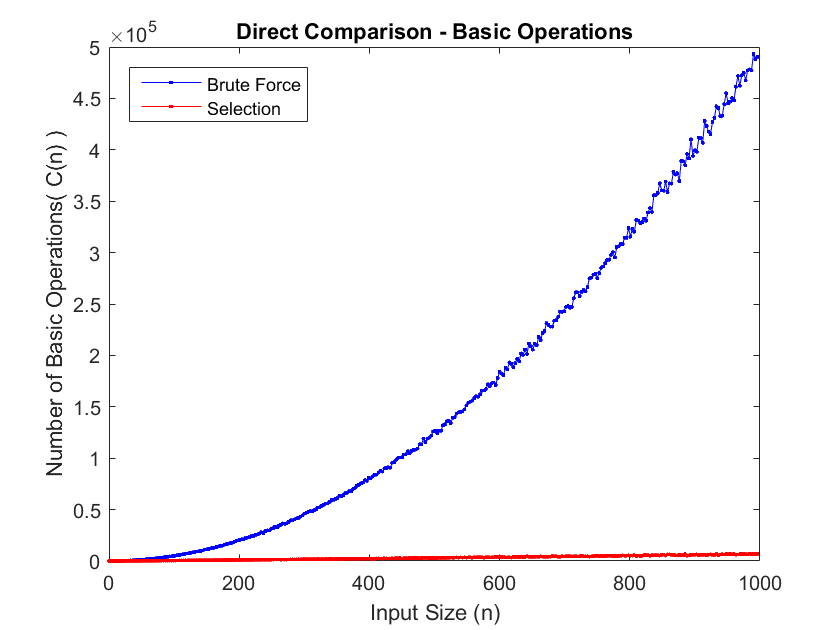
\includegraphics[scale=0.5]{Images/direct_comparison_basic_operations.png}\\
\end{center}
\begin{bottompar}
We declare that we have both contributed equally to this piece of assesment.\\\\\\\\
\noindent\begin{tabular}{ll}
\makebox[2.5in]{\hrulefill} & \makebox[2.5in]{\hrulefill}\\
Jason Queen & Date\\[8ex]% adds space between the two sets of signatures
\makebox[2.5in]{\hrulefill} & \makebox[2.5in]{\hrulefill}\\
Luke Josh & Date\\
\end{tabular}
\end{bottompar}
\newpage
\small{\tableofcontents}
\newpage


\section{Summary}
    The purpose of this report is to analyse and compare the average complexity of the selection median algorithm against a brute force solution. This report uses algorithm analysis techniques to experimentally determine the average case efficiency of both the selection median and a brute force algorithm. The expected theoretical efficiencies of the algorithms are evaluated using mathematical analysis and are contrasted against the computed experimental results. The results for each algorithm are also compared to each other and the most efficient algorithm is determined.

\section{Description of the Algorithms}
    \subsection{Brute Force}
        The brute force median algorithm works by manually checking each value of the array and determining if the element's position in a sorted array is in the median position of $\frac{n}{2}$. It does this by checking each element of the array against every other element of the array, and counting the number of elements that are less than the value, and the number of elements that are greater than the value.

        Recalling that the median value of a list of numbers is the element that occurs in center position (rounded up for the purpose of this algorithm), the algorithm tests if a value is the median value by testing if half the elements in the array are less than the value. This can be seen in the pseudocode included in the next section.

        \subsubsection{The Algorithm}
            \begin{algorithm}[H]
                \caption{Brute Force Median}
                \begin{algorithmic}[1]
                    \Function{BruteForceMedian}{$A[0..n - 1]$}
                        \State{$k \leftarrow \|n / 2\|$}
                        \For{$i \leftarrow 1$ \bf{to} $n - 1$}
                            \State{$numsmaller \leftarrow 0$}
                            \State{$numeqal \leftarrow 0$}
                            \For{$j \leftarrow 0$ \bf{to} $n - 1$}
                                \If{$A[j] < A[i]$}
                                    \State{$numsmaller \leftarrow numsmaller + 1$}
                                \Else
                                    \If{$A[j] = A[i]$}
                                        \State{$numequal \leftarrow numequal + 1$}
                                    \EndIf
                                \EndIf
                            \EndFor
                            \If{$numsmaller < k$ \bf{and} $k \leq (numsmaller + numequal)$}
                                \State{\bf{return} $A[i]$}
                            \EndIf
                        \EndFor
                    \EndFunction
                \end{algorithmic}
            \end{algorithm}

    \subsection{Median Selection Algorithm}
        The selection algorithm for finding the median value of the array derives much of its logic from the QuickSelect algorithm. QuickSelect implements a random selection of a pivot element, which is used to partially sort the array around that pivot - which it then recursively continues on the sub array containing the median. QuickSelect has been quoted to have an average running complexity of $\Theta{n}$ \cite{cormen} - which is a value we can expect to get for the median selection algorithm.

        The selection algorithm uses a recursive method to determine the median of the array.  The recursive function first performs a partition on the array where all elements less than a pivot element (starting with element 0 as the first pivot) are swapped until the pivot element swapped into its correct position. All elements with an index lower than that of the pivot now also have a value which is less than that of the pivot. If the new position of the pivot is the middle of the array then the value of the pivot is returned, as it is the median of the array. This check is the basis for the recursive operation.

        Otherwise, if the position of the pivot is less than or greater than that of the middle index then the recursive function is called again and then performs the partition on either the lower or upper partition of the array respectively. This is performed until the pivot value's index tells us that it is the median.\\
        It should be noted that there is no guarantee that the whole array will be completely sorted by this process. However, all elements at a lower index than that of the pivot will have a value that is lower than that of the pivot element and all elements with an index greater than that of the pivot element will have values that are also greater than the value of the median.

        As opposed to the brute force algorithm, when this algorithm is performed on an array with an even number of elements, the centre value is rounded down - e.g., an array of size 6 would have the 3rd element as its median value.

        An example of this process is as follows, on an array $A = [3, 5, 4, 2, 1]$:\\

        \noindent$A = [3, 5, 4, 2, 1] \rightarrow$  5 and 4 are both greater than 3, do nothing\\\\
        $A = [3, 2, 4, 5, 1] \rightarrow$  $2 < 3$, swap 5 with 2\\\\
        $A = [3, 2, 1, 5, 4] \rightarrow$  $1 < 3$, swap 4 with 1\\\\
        $A = [1, 2, 3, 5, 4] \rightarrow$  Finally, swap 3 with 1\\

        If the first value happens to be the median value of the array, the algorithm stops. However, if the index returned is not the median index, there are two possibilities:

        \begin{enumerate}
            \item If the index is less than the median index, the same process as above is performed, ignoring the first element of the array.
            \item If the index is greater than the median index, the same process as above is performed, ignoring the last element of the array.
        \end{enumerate}

        This process continues until the value with an index equal to the median index is found.

        \subsubsection{The Algorithm}
            \begin{algorithm}[H]
                \caption{Selecion Median}
                \begin{algorithmic}[1]
                    \Function{Median}{$A[0..n - 1$}
                        \If{$n = 1$}
                            \State{\bf{return} $A[0]$}
                        \Else
                            \State{Select($A, 0, |n/2|, n - 1$)}
                        \EndIf
                    \EndFunction\\

                    \Function{Select}{$A[0..n - 1], l, m, h$}
                        \State{$pos \leftarrow$ Partition($A, l, h$)}
                        \If{$pos = m$}
                            \State{\bf{return} $A[pos]$}
                        \EndIf
                        \If{$pos > m$}
                            \State{\bf{return} Select($A, l, m, pos - 1$)}
                        \EndIf
                        \If{$pos < m$}
                            \State{\bf{return} Select($A, pos + 1, m, h$)}
                        \EndIf
                    \EndFunction\\

                    \Function{Partition}{$A[0..n - 1], l, h$}
                        \State{$pivotval \leftarrow A[l]$}
                        \State{$pivotloc \leftarrow l$}

                        \For{$j \leftarrow l + 1$ \bf{to} $h$}
                            \If{$A[j] < pivotval$}
                                \State{$pivotloc \leftarrow pivotloc + 1$}
                                \State{swap($A[pivotloc], A[j]$)}
                            \EndIf
                            \State{swap($A[l], A[pivotloc]$)}
                        \EndFor
                    \State{\bf{return} $pivotloc$}
                    \EndFunction
                \end{algorithmic}
            \end{algorithm}


\section{Theoretical Analysis of the Algorithms}
    \subsection{Choice of Problem Size}
        The algorithms are tested using randomly generated arrays of sizes 1 through to 999 in steps of 3. The test for each array size is repeated 2000 times in order to normalize the results.

        For the selection median, a single array needs to be sorted a number of times to get an accurate measure of the running time - as it runs so quickly that a single test does not return useful or accurate data. For each array size, 2000 random arrays are generated, and the times to run each algorithm are recorded. To combat the extremely quick running time of the selection algorithm, the running time is averaged over 10 runs on each of the same random array - as opposed to the single time it is run for the brute force implementation.

        The upper limit was chosen as array sizes greater than 1000 have brute force time complexities which are significantly large. This limits the number of averages that can be taken for each array size as the total time to run all tests increases to a value that is impractical to perform repeatedly. 

        The odd step size of 3 is chosen so that tests are performed for both odd and even array sizes.
    \subsection{Brute Force Median}
        \subsubsection{Choice of Basic Operations}
            The operation that best defines the complexity and running time of the brute force median algorithm is the comparison $A[j] < A[i]$. This comparison operation is performed more than any other operation in the algorithm - a minimum of $n - 1$ times, and a maximum of $(n - 1)^2$ times.

        \subsubsection{Average Case Efficiency}
            The average case efficiency of the algorithm can be derived by considering then number of operations required to determine the median of an arbitrarily sized array. Consider an array $A = [a_1, a_2, ..., a_(n)]$ with it's median value placed at position $k$. The algorithm must check each element in the array up to and including $A[k]$ against each element in the array, including itself. Thus, the algorithm must perform $k \cdot n$ comparisons to determine that $A[k]$ is the median value of the array.

            To determine the average number of operations for an array of size $n$, we must consider the parity of the size of the array, as the algorithm chooses the value to the left of the midpoint when there are an even number of elements. We will first assume that each value in the array has an equivalent chance of being the median. In this case, the average case number of operations to determine the median is average number of operations over each possibility of the median, M, which can be expressed as $average(M = A[j])$ $\forall j \in [0, 1, ..., n - 1]$:

            \begin{align}
                & c_{average} = \frac{\sum_{j = 1}^{n} j \cdot n}{n} \\
                & c_{average} = \sum_{j = 1}^n j\\
                & c_{average} = \frac{n^2 + n}{2}
            \end{align}

            To account for the issue of parity, consider two sorted arrays, $A = [a_1, a_2, ..., a_n]$ and $B = [a_1, a_2, ..., a_{n+1}$, where $n$ is odd. In each of these arrays, the median value will be the same, $M = a_{floor(\frac{n}{2})}$, and will have to check the same number of elements to find it, however, in $B$, each element is checked against $n + 1$ other elements, as opposed to A's $n$ other elements. We can use this to restate the above value for the average number of comparisons as $c_{odd} = \frac{n^2 + n}{2}$, and conversely, $c_{even} = \frac{n^2}{2}$. These two statements can be combined using a modulo operator to give the true average number of comparisons for an arbitrarily sized array as:
            \begin{align}
                c_{average} = \frac{n^2 + (n\mod 2) \cdot n}{2}
            \end{align}
            Which gives the algorithm an average case complexity of $\Theta(n^2)$.\\
            The above calculations are assuming that all values in an array are unique. In other cases, an array may take the form $[1, 2, 3, 3, 3, 4, 5]$, which will skew the results for the average number of comparisons. For example, an array $A = [1, 2, 4, 5, 3, 3, 3]$, the median value is 3, but 3 appears more than once. This means the algorithm will find the median at the 5th position, but it must check each value against 7 other values.

    \subsection{Selection Median}
        \subsubsection{Choice of Basic Operations}
            The operation that best defines the complexity and running time of the selection median algorithm is the comparison $A[j] < pivotval$ which is performed by the partition sort logic borrowed from the QuickSort algorithm. This comparison operation is performed more than any other operation in the algorithm - a minimum of $n - 1$ times if the median value is in the first position of the array, and a maximum of $(n - 1)^2$ times, if the median value is in its correct position at the centre of the array.

        \subsubsection{Average Case Efficiency}
            The average case number of comparisons performed in the selection algorithm is considerably more complex than that of the brute force implementation. It has been stated that the selection algorithm is extremely similar to the QuickSort algorithm - and as such, a similar computational complexity is expected. Berman and Paul state that the average number of comparisons for an array of size n is less than $4\cdot n$ \cite{kenneth2004}.

\section{Methodology, Tools and Techniques}
    \subsection{Programming Environment}
        All testing and computation was executed on a Microsoft Surface running Windows 8.1 64 bit, Intel Core i5 Processor (1.9GHz), 4GB DDR4 RAM.
        \subsection{Implementation of the Algorithms}
        The algorithms and their tests were both implemented in C++, compiled using the GCC GNU Compiler in the Code Blocks IDE. The source code for these algorithms is included in Appendix 1.

        In general, operation counts were performed by running the algorithm a large number of times on randomly generated arrays, appending the number of operations for each iteration to a pointer to a integer running total, and then calculating the average. The computation time for algorithms was generated in much the same way - using clock types to find the time between two points in the code (namely, the start and end of the algorithm), and then repeating it and taking the average.
 
\section{Experimental Results}
    All graphs referenced in this section have been included in section 1 of the appendix.
    \subsection{Functional Testing}
        To ensure the functional correctness of the implemented algorithms - a number of unit tests have been implemented. These tests are included the the test.cpp file, which is also included in appendix 1. These unit tests ensure that the algorithms produce the expected results for a number of predefined test cases. The output of the test cases for the configuration of the algorithms is as follows:\\\\
        Would you like to run the tests? (0 = No, 1 = Yes)
        1\\
        Test 1\\
        \tab Array = [ 1 2 3 4 5 ]\\
        \tab \tab Brute Force Algorithm\\
        \tab \tab \tab Num Operations = 15\\
        \tab \tab \tab Answer = 3\\
        \tab \tab \tab Expected = 3\\
        \tab \tab \tab Passed = 1\\
        \tab \tab Selection Algorithm\\
        \tab \tab \tab Num Operations = 9\\
        \tab \tab \tab Answer = 3\\
        \tab \tab \tab Expected = 3\\
        \tab \tab \tab Passed = 1\\
        \tab Passed = 1\\
        Test 2\\
        \tab Array = [ 1 2 3 4 5 6 ]\\
        \tab \tab Brute Force Algorithm\\
        \tab \tab \tab Num Operations = 18\\
        \tab \tab \tab Answer = 3\\
        \tab \tab \tab Expected = 3\\
        \tab \tab \tab Passed = 1\\
        \tab \tab Selection Algorithm\\
        \tab \tab \tab Num Operations = 14\\
        \tab \tab \tab Answer = 4\\
        \tab \tab \tab Expected = 4\\
        \tab \tab \tab Passed = 1\\
        \tab Passed = 1\\
        Test 3\\
        \tab Array = [ 1 2 3 3 5 ]\\
        \tab \tab Brute Force Algorithm\\
        \tab \tab \tab Num Operations = 15\\
        \tab \tab \tab Answer = 3\\
        \tab \tab \tab Expected = 3\\
        \tab \tab \tab Passed = 1\\
        \tab \tab \tab Selection Algorithm\\
        \tab \tab \tab Num Operations = 9\\
        \tab \tab \tab Answer = 3\\
        \tab \tab \tab Expected = 3\\
        \tab \tab \tab Passed = 1\\
        \tab Passed = 1\\
        Which shows that the algorithms are functionally correct, and do return the median value of the test arrays.
    \subsection{Brute Force}
        \subsubsection{Number of operations}
            The number of operations of the brute force median algorithm was calculated by running the algorithm on a random array of various sizes, and counting the number of times the comparison $A[j] < A[i]$ is performed. This expected number of comparisons was calculated above to be $\frac{n^2}{2}$ for odd sized arrays, and $\frac{n^2 + n}{2}$ for even sized arrays. This function has been graphed along the data that was collected from the tests, and is included as the first figure of section 7.1.1, and clearly shows that the expected trend holds true.

            It must be noted that the data sets used to test the number of operations is not tested for uniqueness - a single value may appear more than once. This causes some amount of discrepancy between the expected result and the actual result, but can mostly be corrected by increasing the maximum value of the random generated numbers to be sufficiently large. This can be seen in the source code in section 6.1.4, on line 97.
        \subsubsection{Computation time}
            The computation for the brute force algorithm was expected to run in $\Theta{n^2}$ time. In other words, the time for the algorithm to run is determined quadratically by the number of elements in the array. It can be seen in the the second figure of section 7.7.1 that the collected data follows a quadratic trend. Included on this graph also is the operation count again, which allows us to see that the average case running time is indeed correlated to the number of basic operations performed.

    \subsection{Selection}
        \subsubsection{Number of operations}
            The selection algorithm was quoted to perform less than $4 \cdot n$ comparisons to determine the median value of array of size n on average. For comparison, the line $comparisons = 4 \cdot array\_size$ has been graphed, and is included as the first figure in section 7.1.2. It is clear that the recorded data fits the expected trend - as it on average lies below the line. As the number of samples or averages is increased, the variance would become less, and the recorded data would trend closer and closer to a straight line which lies underneath the plotted function.
        \subsubsection{Computation time}
            An operating complexity of $\Theta{n}$ was expected for the median selection. The graph included (second figure of section 7.1.2) of this data makes the linear trend clear - especially when compared to the quadratic expected value for the brute force algorithm.

    \subsection{Comparison}
        As the two algorithms perform the same operation, they are able to be quantitatively compared. In section 3, we have theoretically shown that the average computational complexity of the brute force and selection algorithms are $\Theta{n^2}$ and $\Theta{n}$ respectively. In section 5, we have shown that these theoretical models fit the data that was collected quite well - which allows us to confidently compare the two algorithms.

        It is clear that the selection algorithm is superior to the brute force method for an arbitrarily sized array - shown computationally and analytically. Included as section 7.1.3 are graphs comparing the computation time and operation count for both algorithms, these allow us to see the drastic difference between these two (result wise) equivalent algorithms. It can be seen that the difference in linear and quadratic running time causes the brute force method to reduce the selection method to less than a percent of the graphs y axis.
\section{Conclusion}
    In this report, the average case efficiency of the Brute Force Median and Selection Median algorithms are analytically and experimentally compared. Through mathematical and experimental analysis, the Brute Force algorithm is identified to have an average case efficiency which follows a quadratic trend. The second algorithm, the Selection Median, is determined to follow a linear trend. These identified trends hold true for both the basic operation and time complexities. Comparatively, the average case efficiency of the Selection Median algorithm is always less than that of the Brute Force Median implementation. 

    Thus, on average, the Selection Median is determined to be a more efficiency algorithm than the Brute Force Median algorithm.
\newpage
\section{Appendix}
    \subsection{Figures}
        \subsubsection{Brute Force}
            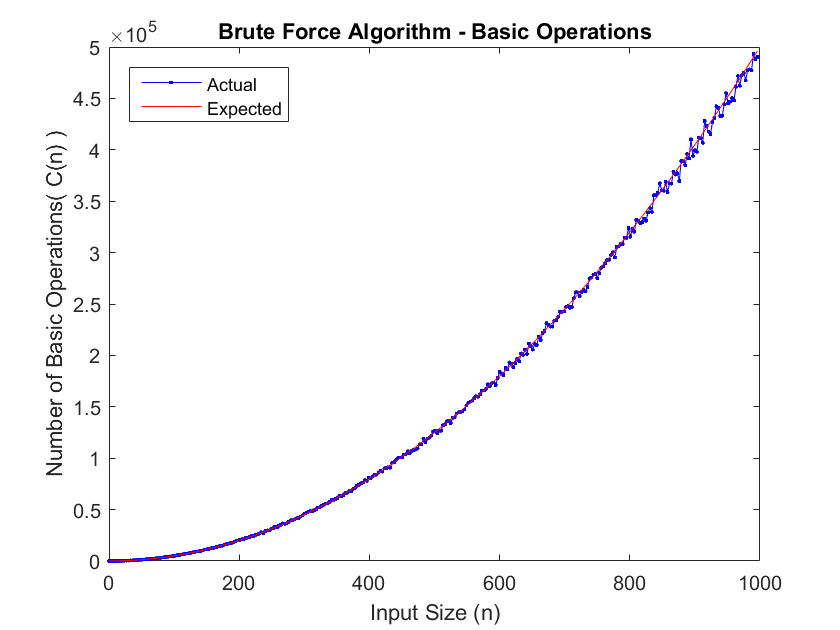
\includegraphics[scale=0.6]{Images/brute_algorithm_basic_operations.png}\\
            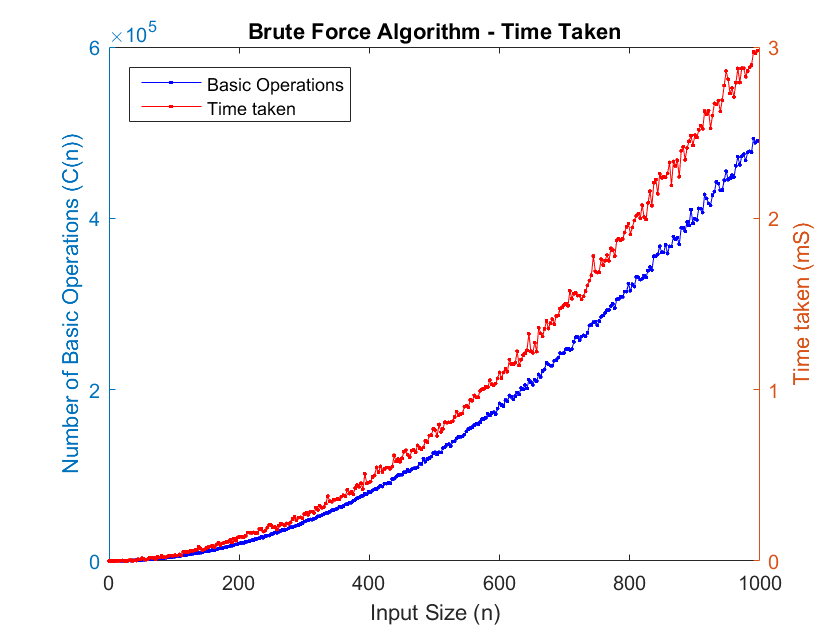
\includegraphics[scale=0.6]{Images/brute_algorithm_time_taken.png}
        \subsubsection{Selection}
            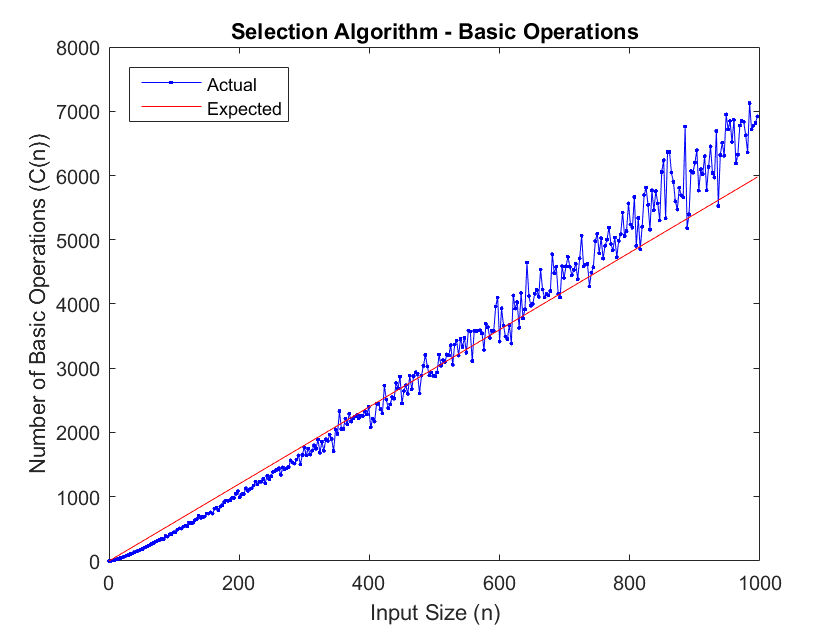
\includegraphics[scale=0.6]{Images/selection_algorithm_basic_operations.png}\\
            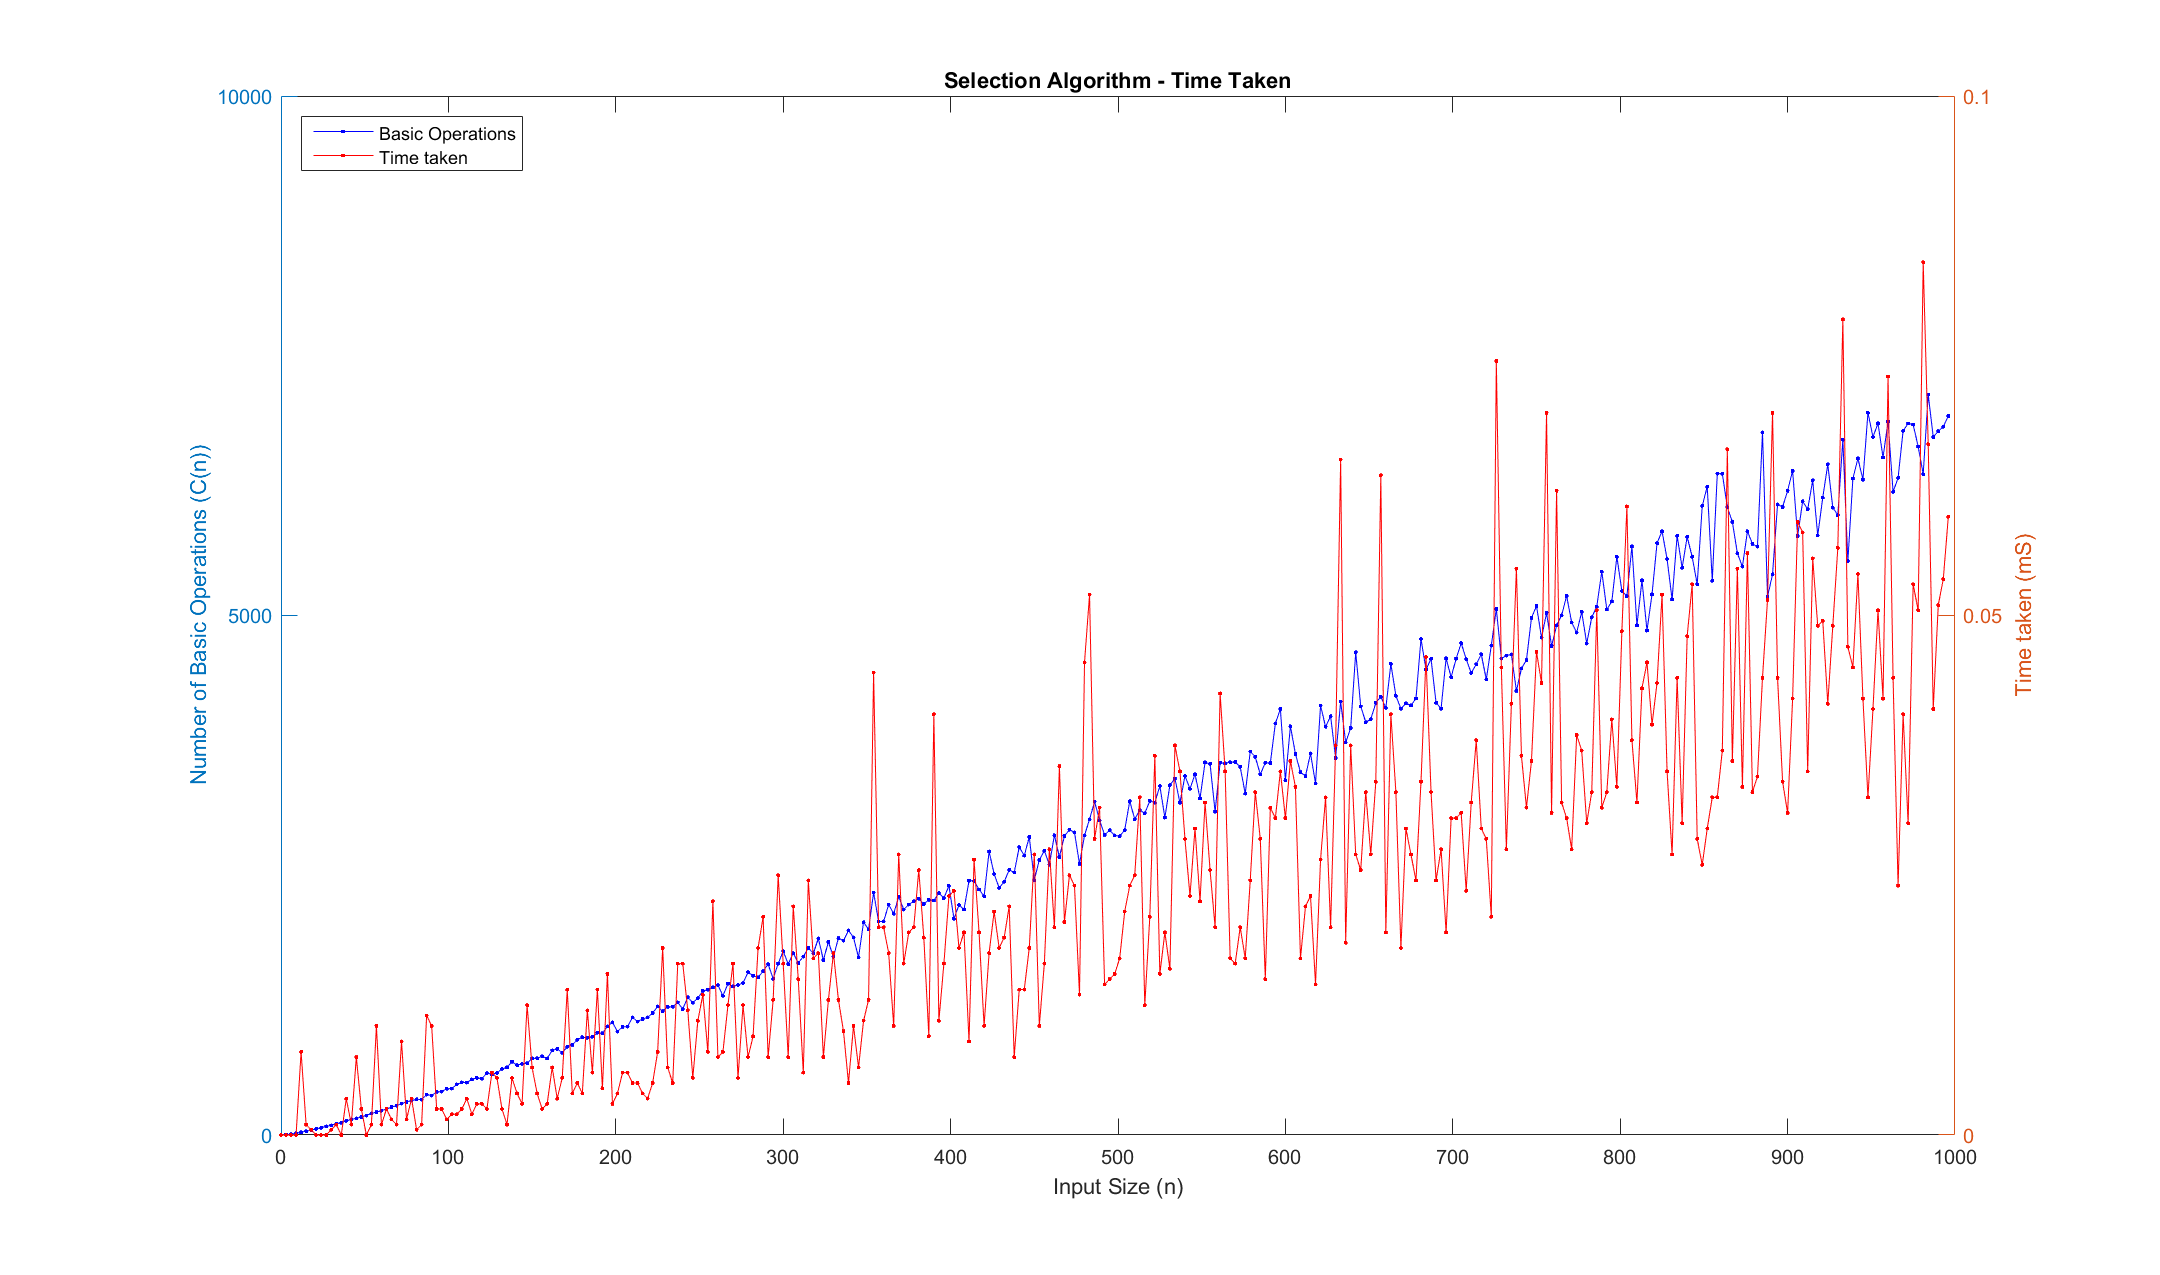
\includegraphics[scale=0.6]{Images/selection_algorithm_time_taken.png}
        \subsubsection{Comparison}
            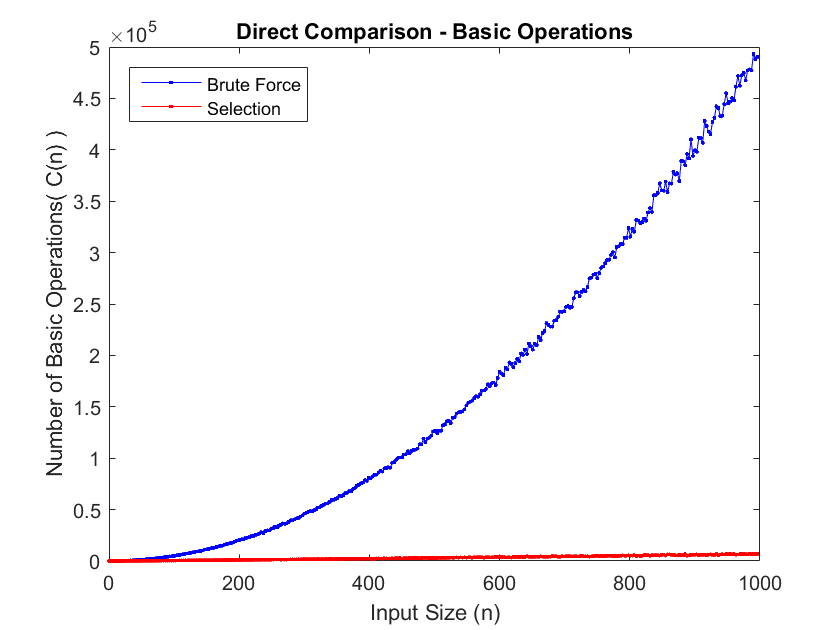
\includegraphics[scale=0.6]{Images/direct_comparison_basic_operations.png}\\
            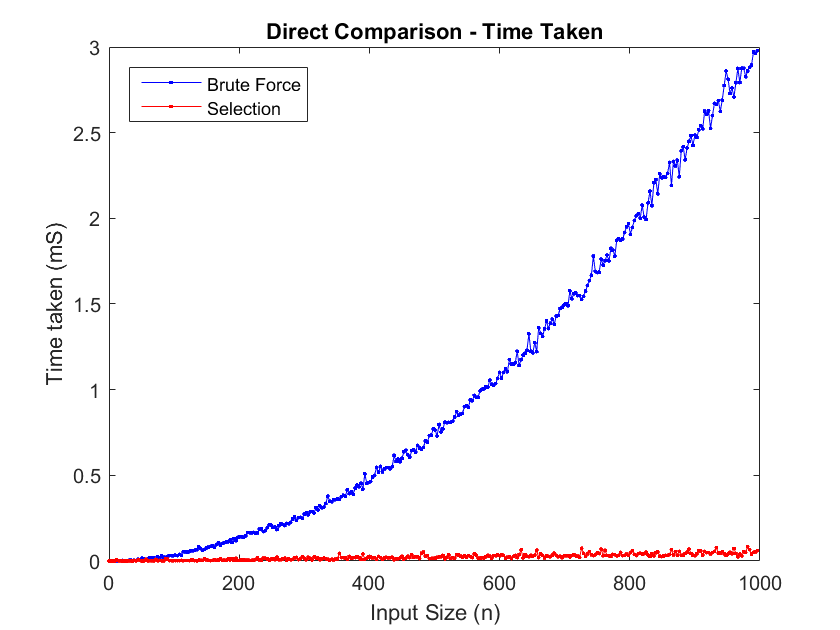
\includegraphics[scale=0.6]{Images/direct_comparison_time_taken.png}
    \newpage
    \subsection{Source Code}
        \subsubsection{Brute Force Median}
            \lstinputlisting[language=C++]{CAB301_Assignment2/bruteForceMedian.cpp}

        \subsubsection{Selection Median}
            \lstinputlisting[language=C++]{CAB301_Assignment2/selectionMedian.cpp}

        \subsubsection{Main}
            \lstinputlisting[language=C++]{CAB301_Assignment2/main.cpp}

        \subsubsection{Unit Tests}
            \lstinputlisting[language=C++]{CAB301_Assignment2/tests.cpp}
        \subsubsection{Matlab Graphing}
            \lstinputlisting[language=Matlab]{CAB301_Assignment2/MATLAB_plotting_program.m}
        \newpage
\section{Bibliography}
    \bibliography{bibliography}
\end{document}